\begin{figure}[H]
  \centering
  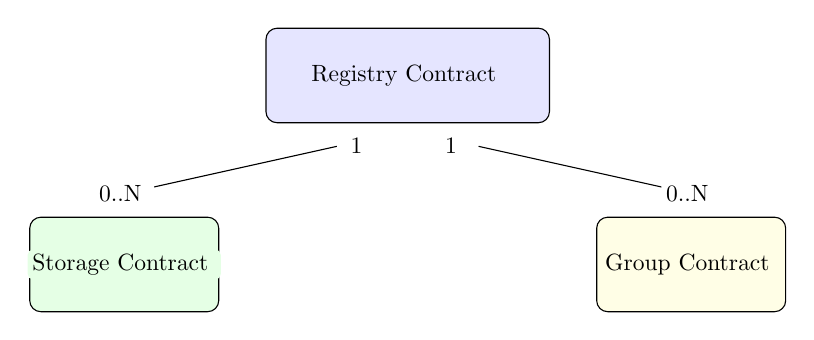
\begin{tikzpicture}[scale = 0.6, every node/.style={scale = 0.85}, every node/.append style={fill = white, rounded corners = 2pt, inner sep = 2pt, align = center}]

  \draw [rounded corners, fill=blue!10] (-3, 2) rectangle (3, 0);
  \node [fill=blue!10] at (0, 1) { Registry Contract };

  \draw [rounded corners, fill=green!10] (-8, -4) rectangle (-4, -2);
  \node [fill=green!10] at (-6, -3) { Storage Contract };

  \draw [rounded corners, fill=yellow!10] (4, -4) rectangle (8, -2);
  \node [fill=yellow!10] at (6, -3) { Group Contract };

  \draw (-1.5,  -0.5) -- (-6,  -1.5);
  \node at (-1, -0.5) { 1 };
  \node at (-6, -1.5) { 0..N };

  \draw (1.5,  -0.5) -- (6,  -1.5);
  \node at (1, -0.5) { 1 };
  \node at (6, -1.5) { 0..N };

  \end{tikzpicture} \\
  \caption{
  	Ethereum Micro-Architecture
  }{
    Outline of the micro-architecture of Ethereum contracts, shown with cardinality.
  }
  \label{fig:ethereum_micro_architecture}
\end{figure}
